\chapter{Ličnost Boga - Članak James S. Whitea}

U nastavku ćemo pregledati pamflet Jamesa Whitea pod nazivom “\textit{Ličnost Boga}”. Čitajući ovaj članak, prepoznat ćemo da James White nastavlja tamo gdje je brat Loughborough stao i da proširuje i produbljuje razumijevanje koje stoji iza prve točke \emcap{Fundamentalnih Principa}.

Traktat Jamesa Whitea tiskan je više puta, oglašavan je 54 puta i dva puta ponovno objavljen u publikaciji Review and Herald. Njegovo gledište o \emcap{ličnosti Boga} bilo je dobro poznato i široko rasprostranjeno unutar adventizma. U ovom pamfletu vidjet ćemo jasnu kritiku prema idejama koje je Kellogg zagovarao u Živom Hramu.

\begin{figure}[hp]
    \centering
    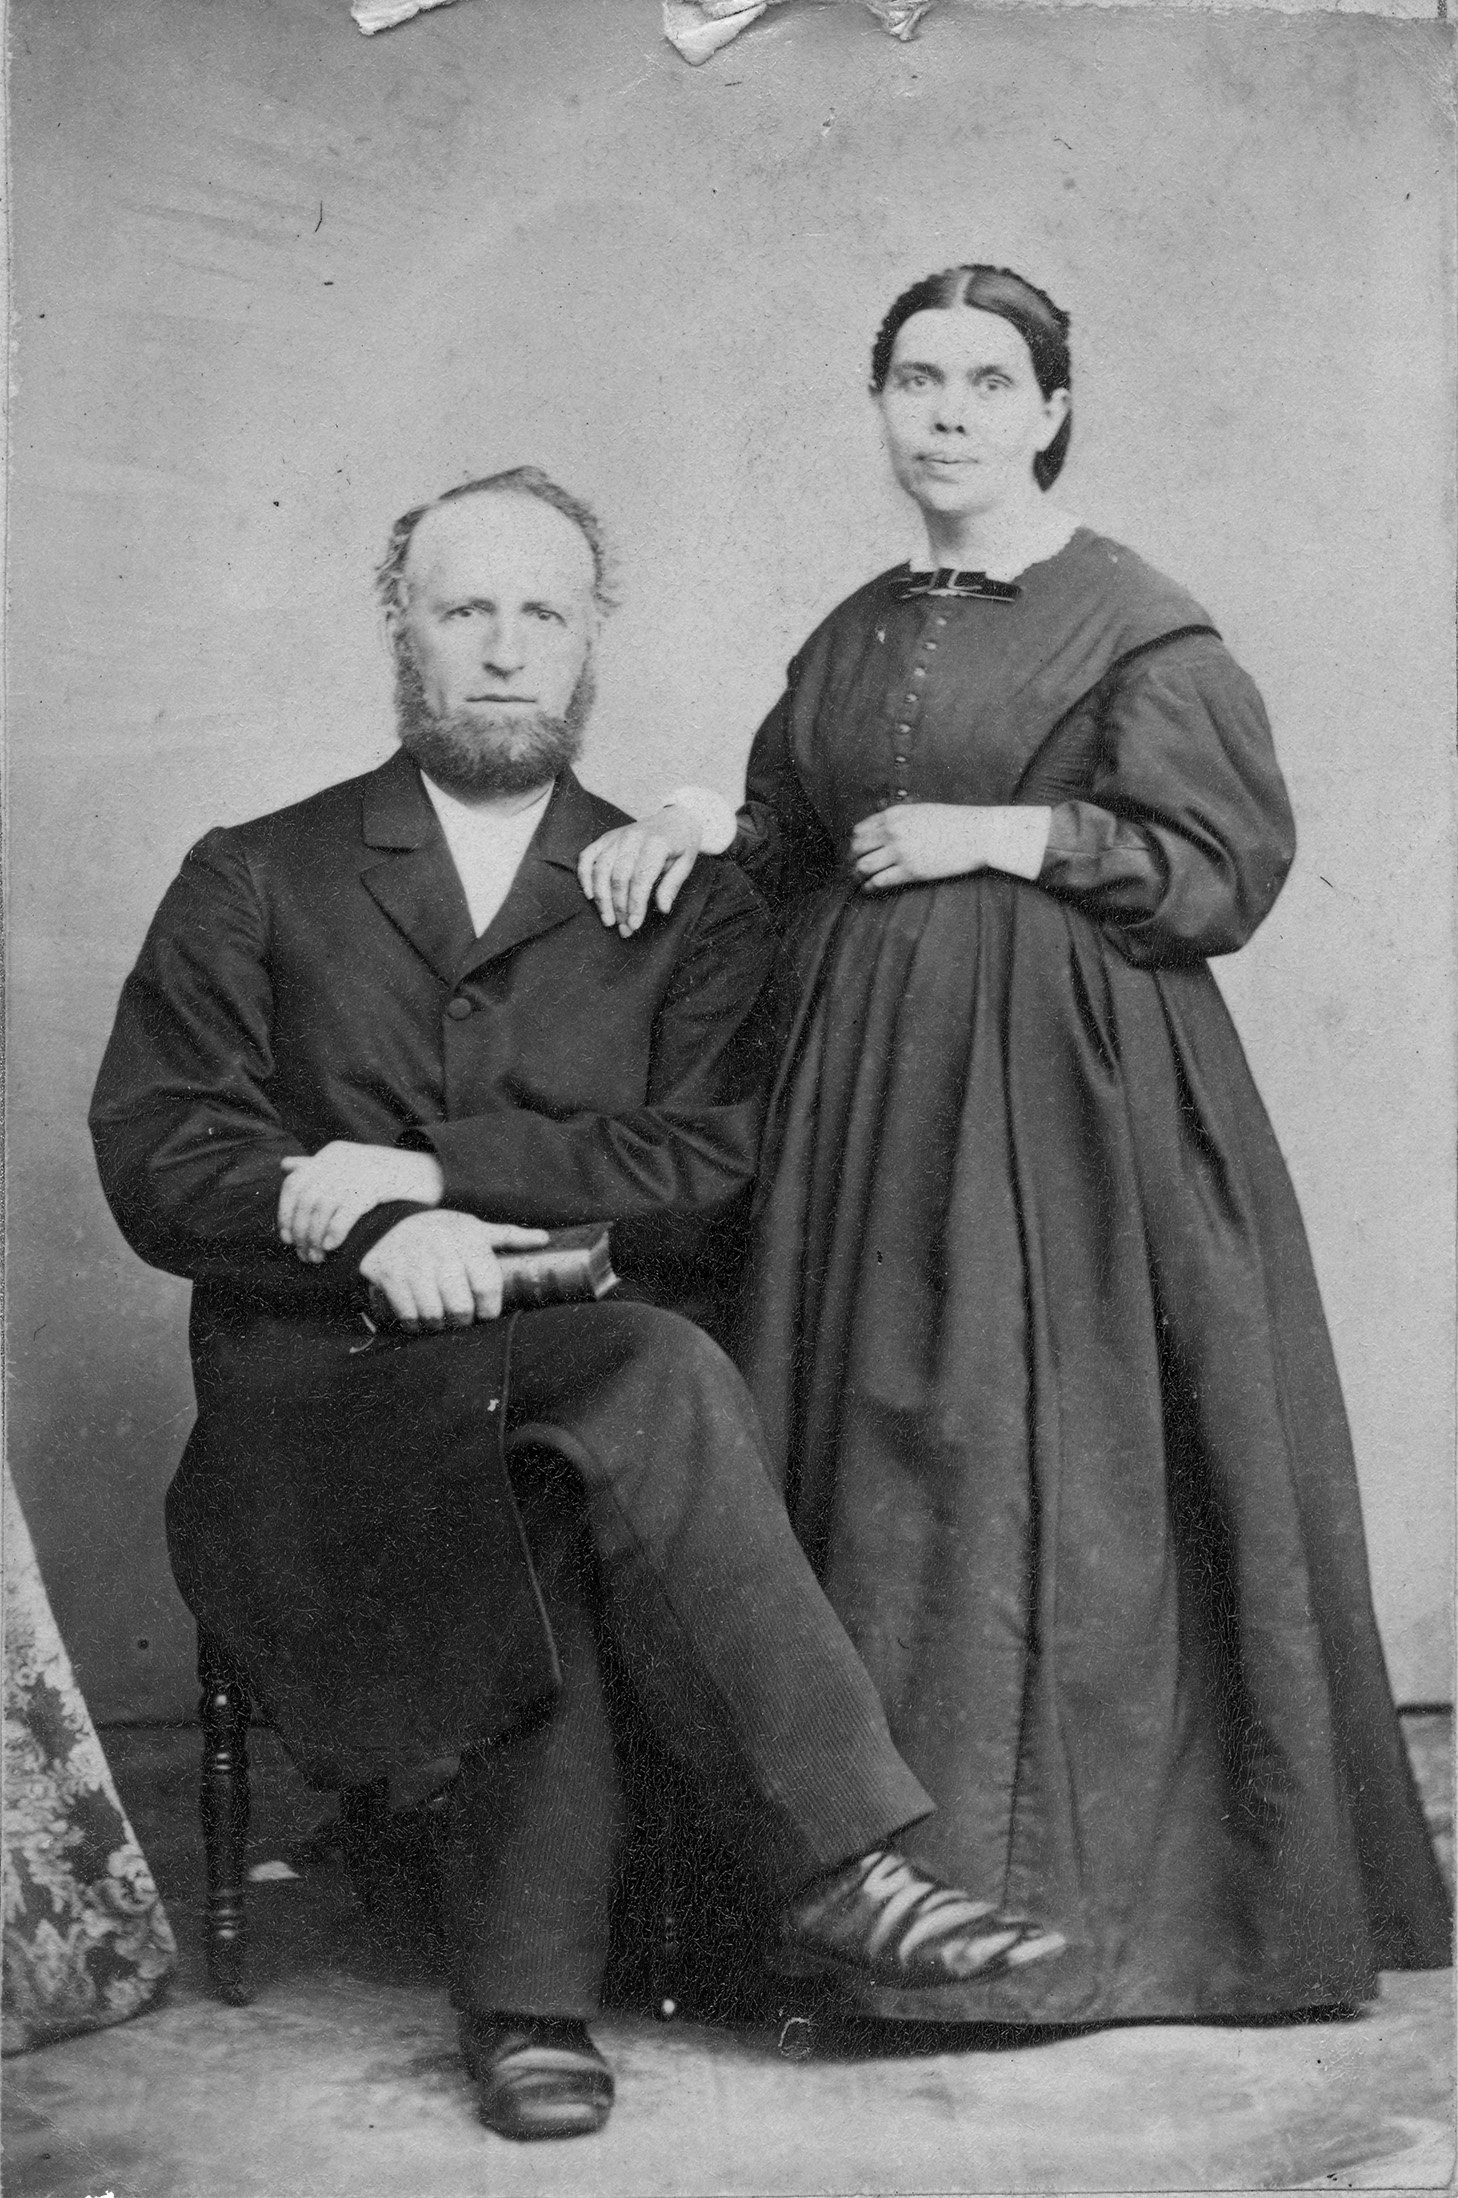
\includegraphics[width=1\linewidth]{images/james-and-ellen-white.jpg}
    \caption*{James Springer White (1821-1881) i Ellen White (1827-1915)}
    \label{fig:james-and-ellen-white}
\end{figure}

\othersQuote{\textbf{ČOVJEK je stvoren na sliku Božju}. ‘I reče Bog: Stvorimo čovjeka na našu sliku, nama sličnoga’. ‘Tako Bog stvori čovjeka na svoju sliku, na sliku Božju stvori ga.’ Postanak 1:26, 27. Vidi također poglavlje. 9:6; 1. Korinćanima 11:7. \textbf{Oni koji poriču ličnost Boga, kažu da ‘slika’ ovdje ne znači \underline{fizički oblik}, već moralnu sliku, i to čine glavnom polaznom točkom za dokazivanje besmrtnosti svih ljudi}. Argument ide ovako: Prvo, čovjek je stvoren na Božju moralnu sliku. Drugo, Bog je besmrtno biće. Treće, stoga su svi ljudi besmrtni. Ali ovaj način razmišljanja također bi dokazao da je čovjek svemoćan, sveznajući i sveprisutan, i tako obukao smrtnog čovjeka u sve atribute božanstva. Pokušajmo: Prvo, čovjek je stvoren na Božju moralnu sliku. Drugo, Bog je svemoguć, sveznajući i sveprisutan. Treće, dakle, čovjek je svemoguć, sveznajući i sveprisutan. Ono što dokazuje previše, ne dokazuje ništa, stoga se stajalište da Božja slika znači njegovu moralnu sliku ne može održati. \textbf{Kao dokaz da je Bog osoba, pročitajte njegove riječi Mojsiju}: ‘I reče Gospod: »Evo mjesta uza me, a ti stani na stijenu. I dogodit će se, dok moja slava bude prolazila, da ću te staviti u raspuklinu stijene i \textbf{svojom te rukom} zakloniti dok \textbf{ne prođem}. Onda ću \textbf{ruku svoju} maknuti, pa ćeš me \textbf{vidjeti odostrag}; \textbf{ali se lice moje ne može vidjeti}.’ Izlazak 33:21-23. Vidi također poglavlje. 24:9-11. \textbf{Ovdje Bog govori Mojsiju da će \underline{vidjeti njegov oblik}}. \textbf{Reći da je Bog učinio da se Mojsiju čini kako vidi njegov oblik, kada on nema oblik, znači optužiti Boga da je uz neistinu dodao i neku vrstu mađioničarske obmane svom sluzi Mojsiju}.}[James S. White, PERGO 1.1; 1861][https://egwwritings.org/read?panels=p1471.3]

\othersQuoteNoGap{No skeptik misli da vidi proturječje između 11. stiha, koji kaže da je Gospod govorio Mojsiju licem u lice, i 20. stiha, koji kaže da Mojsije nije mogao vidjeti njegovo lice. Ali neka Brojevi 12:5-8 otklone poteškoće. ‘\textbf{Tada Gospod siđe u stupu od oblaka}, te stane na ulaz u Šator i zovne Arona i Mirjam. I njih dvoje istupiše. Onda reče: Počujte sad riječi moje: Nađe li se prorok među vama, ja, Gospod, u viđenju se njemu javljam, u snu njemu progovaram. Nije tako sa slugom mojim Mojsijem, on je vjeran u svemu domu mojemu. \textbf{Ustima u usta njemu progovaram, i to \underline{jasno}}.’}[James S. White, PERGO 2.1; 1861][https://egwwritings.org/read?panels=p1471.6]

\othersQuoteNoGap{Veliki i strašni Bog je sišao, obavijen oblakom slave. \textbf{Taj se oblak mogao vidjeti, ali ne i lice koje ima blistaviju svjetlinu od tisuću sunaca}. Pod tim okolnostima, Mojsiju je bilo dopušteno da se približi i \textbf{razgovara s Bogom licem u lice, ili usta na usta, čak i \underline{naizgled}}.}[James S. White, PERGO 2.2; 1861][https://egwwritings.org/read?panels=p1471.7]

\othersQuoteNoGap{Prorok Daniel kaže: ‘Gledao sam sve dok prijestolja ne bijahu zbačena i \textbf{Drevnik vjekova ne sjede}, odjeća mu bijaše bijela kao snijeg, \textbf{a kosa na glavi njegovoj kao čista vuna}; \textbf{prijestolje mu kao plamenovi ognjeni, a kotači mu kao rasplamsali oganj}.’ Poglavlje 7:9. ‘Gledah u noćnim viđenjima, i gle, netko nalik Sinu Čovječjemu dolažaše s oblacima nebeskim i \textbf{dospije do Drevnika vjekova}, i \textbf{dovedoše ga preda nj}, i njemu bȋ predana vlast i slava i kraljevstvo.’ Stihovi 13, 14.}[James S. White, PERGO 2.3; 1861][https://egwwritings.org/read?panels=p1471.8]

\othersQuoteNoGap{Ovdje je uzvišen opis djelovanja \textbf{dviju osoba}; naime, \textbf{Boga Oca i njegovog Sina Isusa Krista}. \textbf{Poreknete li njihove ličnosti, više nemate jasan smisao u ovim citatima iz Daniela}. U vezi s ovim citatom pročitajte izjavu apostola da je \textbf{Sin bio savršena slika osobe svog Oca}. ‘Mnogo puta i na mnogo načina Bog negda progovori ocima po prorocima, a u ovim posljednjim danima progovori nama po Sinu, kojega postavi baštinikom svega, po kojemu i sazda svjetove; \textbf{on, koji je odsjaj slave i savršena slika njegove osobe}.’ Hebrejima 1:1-3.}[James S. White, PERGO 3.1; 1861][https://egwwritings.org/read?panels=p1471.11]

\othersQuoteNoGap{Mi ovdje dodajemo Kristovo svjedočanstvo. ‘I sam Otac, koji me posla, svjedoči za mene. Niti ste čuli njegov glas ikada \textbf{niti ste vidjeli njegov oblik}.’ Ivan 5:37. Vidi i Filipljanima 2:6. \textbf{Reći da Otac nema osobni oblik, čini se da je najizraženija kontradikcija jednostavnih izraza iz Svetih pisama}. \\
PRIGOVOR. - ‘\textbf{\underline{Bog je Duh}}.’ Ivan 4:24.}[James S. White, PERGO 3.2; 1861][https://egwwritings.org/read?panels=p1471.12]

\othersQuoteNoGap{ODGOVOR. - \textbf{Anđeli su također duhovi} [Psalam 104:4], ipak oni koji su posjetili Abrama i Lota, legli su, jeli i uhvatili Lotovu ruku. \textbf{Oni su duhovna bića. Tako je i Bog duhovno biće}.}[James S. White, PERGO 3.3; 1861][https://egwwritings.org/read?panels=p1471.13]

\othersQuoteNoGap{PRIGOVOR. - \textbf{Bog je posvuda}. Dokaz. Psalam 139:1-8. \textbf{On je jednako na svakom mjestu kao da je na jednom mjestu}.}[James S. White, PERGO 3.4; 1861][https://egwwritings.org/read?panels=p1471.14]

\othersQuoteNoGap{ODG. - 1. \textbf{Bog je svugdje na temelju svoga sveznanja}, kao što će se vidjeti iz samih riječi Davida. Stihovi 1-6. ‘O Gospode, \textbf{proničeš me i poznaješ}. \textbf{Ti znaš} kada sjednem i kada ustanem, \textbf{prozireš} namisao moju izdaleka. Moju stazu i lijeganje moje ispituješ, i svi moji putovi \textbf{tebi su znani}. Riječ mi još nije na jeziku, kad gle, Gospode, \textbf{svu je znadeš}. Straga i sprijeda ti me obuhvaćaš, i ruku svoju na mene stavljaš. \textbf{Ta spoznaja} odveć mi je čudesna, previsoka je, dokučit’ je ne mogu.’}[James S. White, PERGO 3.5; 1861][https://egwwritings.org/read?panels=p1471.15]

\othersQuoteNoGap{2. \textbf{Bog je \underline{svugdje prisutan svojstvom svoga Duha}, \underline{koji je njegov predstavnik}, i očituje se gdje god mu se svidi}, kao što će se vidjeti na samim riječima koje prigovarač navodi, a koje se spominje gore. Stihovi 7-10. ‘\textbf{Kamo da odem od \underline{Duha tvojega}}? \textbf{i kamo da od \underline{prisutnosti tvoje} pobjegnem}? Ako se popnem na nebo, ti si ondje; ako si u Šeolu prostrem, evo tebe. Uzmem li krila zorina, nastanim li se nakraj mora, i ondje bi me ruka tvoja vodila, i držala me desnica tvoja.’}[James S. White, PERGO 4.1; 1861][https://egwwritings.org/read?panels=p1471.18]

\othersQuoteNoGap{\textbf{Bog je na nebu}. To smo učeni u Gospodinovoj molitvi. ‘\textbf{Oče naš koji jesi na nebesima}’. Matej 6:9; Luka 11:2. \textbf{Ali ako je Bog jednako na svakom mjestu kao da je na jednom mjestu, onda je nebo isto toliko na svakom mjestu kao da je na jednom mjestu, i ideja o odlasku na nebo je zabluda}. Svi smo na nebu; i Gospodinova molitva, prema ovoj maglovitoj teologiji jednostavno znači, Oče naš \textbf{koji jesi svugdje}, sveti se ime tvoje. Dođi kraljevstvo tvoje; budi volja tvoja kako na zemlji, \textbf{tako i svugdje}.}[James S. White, PERGO 4.2; 1861][https://egwwritings.org/read?panels=p1471.19]

\othersQuoteNoGap{Opet, čitatelji Biblije su vjerovali da su Enoh i Ilija doista bili uzeti \textbf{Bogu na nebo}. \textbf{Ali ako su Bog i nebo jednako na svakom mjestu kao na bilo kojem mjestu, sve je onda to zabluda}. Oni nisu bili uzneseni. I sve što je rečeno o vatrenim kolima i vatrenim konjima, i o vihoru koji je došao da odvede Iliju na nebo, bila je beskorisna parada. Oni su samo isparili, a maglovita para prošla je kroz cijeli svemir. To je sve od Enoha i Ilije što um može shvatiti, \textbf{priznajući da Bog i nebo više nisu na jednom mjestu nego na svakom mjestu}. Ali za Iliju se kaže da je ‘\textbf{uzišao} u vihoru \textbf{u nebo}.’ 2 Kraljevi 2:11. O Henoku se kaže da je ‘hodio s Bogom i nestade, jer ga je Bog uzeo.’ Postanak 5:24.}[James S. White, PERGO 4.3; 1861][https://egwwritings.org/read?panels=p1471.20]

\othersQuoteNoGap{\textbf{Za Isusa se kaže da je s desne strane Veličanstva na visini}. Hebrejima 1:3. ‘Tada Gospodin, nakon što im sve to izgovori, \textbf{bȋ uzet \underline{u nebo}}, \textbf{i sjede zdesna Bogu}.’ Marko 16:19. \textbf{Ali ako je nebo posvuda, i Bog posvuda, onda Kristovo uzašašće na nebo zdesna Ocu, jednostavno znači da je on išao svugdje}! On je bio samo odveden tamo gdje ga je oblak sakrio od pogleda svojih učenika, a zatim ispario i otišao svugdje! Tako da umjesto lijepog Isusa, tako lijepo opisanog u oba Zavjeta, imamo samo neku vrstu bîti raspršene po cijelom svemiru. I u skladu s tom razrijeđenom teologijom, Kristov drugi dolazak, ili njegov povratak, bio bi kondenziranje ove bîti na neki lokalitet, recimo na Maslinsku goru! \textbf{Krist je iz mrtvih ustao u fizičkom obliku}. ‘On nije ovdje’, reče anđeo, ‘jer je uskrsnuo kao što je rekao.’ Matej 28:6.}[James S. White, PERGO 5.1; 1861][https://egwwritings.org/read?panels=p1471.23]

\othersQuoteNoGap{‘I dok su išle javiti njegovim učenicima, gle, dođe im ususret Isus govoreći: »Zdravo!« A one pristupe, \textbf{obujme mu noge}, i poklone mu se.’ Stih 9.}[James S. White, PERGO 5.2; 1861][https://egwwritings.org/read?panels=p1471.24]

\othersQuoteNoGap{‘\textbf{Pogledajte moje ruke i noge},’ reče Isus onima koji su sumnjali u njegovo uskrsnuće, ‘ja sam, glavom! \textbf{Opipajte me i vidite, \underline{duh nema tijela i kostiju} kao što vidite da ja imam}.’ ‘\textbf{I to rekavši, pokaza im ruke i noge}. A dok oni još od radosti nisu vjerovali i čudili se, reče im: »Imate li ovdje što za jelo?« A oni mu dadoše komad pečene ribe i meda u saću. On uzme i pojede pred njima.’ Luka 24:39-43.}[James S. White, PERGO 5.3; 1861][https://egwwritings.org/read?panels=p1471.25]

\othersQuoteNoGap{Nakon što se Isus obratio svojim učenicima na Maslinskoj gori, \textbf{on je bio uzet od njih}, i oblak ga je primio izvan njihovih pogleda. ‘I dok su očiju uprtih \textbf{u nebo gledali kako on odlazi}, gle, stadoše kraj njih dva čovjeka u bijeloj odjeći, koji rekoše: »Ljudi Galilejci, što stojite i gledate u nebo? Ovaj Isus koji je \textbf{od vas uzet u nebo}, isto će tako doći kao što ste ga vidjeli da \textbf{u nebo odlazi}«.’ Djela 1:9-11. J. W.}[James S. White, PERGO 6.1; 1861][https://egwwritings.org/read?panels=p1471.27]

James White se bori protiv ideje da je Bog samo duh, i kao takav, prisutan \others{jednako na svakom mjestu kao na bilo kojem mjestu}. On daje jasno i pozitivno svjedočanstvo iz Pisma da je Bog osobno biće; iste sentimente vidimo u spisima Ellen White.

\egw{Moćna sila koja djeluje kroz čitavu prirodu i održava sve što postoji nije, kao što to prikazuju neki znanstvenici, \textbf{samo jedno sveobuhvatno načelo}, jedna pokretačka energija. \textbf{\underline{Bog jeste duh, a ipak je osobno Biće}}, \textbf{jer je čovjek stvoren po Njegovom obličju}. \textbf{Kao \underline{osobno biće}}, Bog je otkrio Sebe u Svojemu Sinu. Isus, odsjaj Očeve slave, “i \textbf{savršena \underline{slika Njegove osobe}}” (Hebrejima 1:3), našao se na zemlji u obličju čovjeka. Kao \textbf{osobni Spasitelj} On je došao na svijet. Kao \textbf{osobni Spasitelj On je uzašao \underline{na visinu}}. Kao \textbf{osobni Spasitelj On posreduje \underline{u nebeskim dvorima}}. \textbf{Pred prijestoljem Božjim} u naše ime služi ‘Nalik Sinu Čovječjemu.’ Daniel 7:13.}[Ed 131.5; 1903][https://egwwritings.org/read?panels=p29.632]

Ellen White i pioniri adventizma napravili su razliku između pojmova ‘\textit{duh}’ i ‘\textit{biće}’. Bog je osobno biće, a ne samo duh. On nije \others{jednako na svakom mjestu kao na bilo kojem mjestu}, nego je\others{na jednom mjestu više nego na drugom}[John. N. Loughborough, “\textit{Is God a Person?}” The Adventist Review and Sabbath Herald, 18. rujna 1855][https://documents.adventistarchives.org/Periodicals/RH/RH18550918-V07-06.pdf]. On je na nebu, u svom hramu, sjedi na svom prijestolju—osobno—i svuda je prisutan preko svog predstavnika, Svetog Duha.

Evo nekoliko drugih citata sestre White koji su u skladu s pogledima pionira po pitanju \emcap{ličnosti Boga}:

\egw{On \normaltext{[Isus]} je učio da je Bog onaj koji nagrađuje pravedne i kažnjava prijestupnike. \textbf{On nije bio neopipljivi duh}, već živi vladar svemira. \textbf{Ovaj milostivi Otac} je neprestano radio za dobro čovjeka i bio je svjestan svega što se njega tiče...}[3SP 47.1; 1878][https://egwwritings.org/read?panels=p142.195]

\egw{\textbf{Biblija nam pokazuje \underline{Boga na Njegovom uzvišenom i svetom mjestu}}, ne u stanju neaktivnosti, ne u tišini i samoći, već okruženog deset tisuća puta deset tisuća i tisuće tisuća svetih bića, koji svi čekaju izvršiti Njegovu volju. \textbf{Preko ovih glasnika On je u aktivnoj komunikaciji sa svakim dijelom svoje vladavine}. \textbf{\underline{Svojim Duhom On je svugdje prisutan}}. \textbf{Kroz djelovanje svog Duha i svojih anđela} On služi djeci ljudskoj.}[MH 417.2; 1905][https://egwwritings.org/read?panels=p135.2136]

\egw{Veličina Božja je za nas neshvatljiva. ‘\textbf{GOSPOD je u svom svetom Hramu}’ (Psalam 11:4); \textbf{\underline{ipak, po svom Duhu je svuda prisutan}}. \textbf{Ima intimno znanje} o, i osobni interes za, sva djela Svoje ruke.}[Ed 132.2; 1903][https://egwwritings.org/read?panels=p29.636]

\egw{Kroz Isusa Krista, \textbf{Bog—ne parfem, \underline{ne nešto neopipljivo}, \underline{već osobni Bog}}—stvorio je čovjeka i obdario ga inteligencijom i moći.}[Ms117-1898.10; 1898][https://egwwritings.org/read?panels=p7182.15]

Nastavljajući s pamfletom Jamesa Whitea, čitamo njegovu oštru kritiku na razumijevanje Boga kao nematerijalnog. Prije toga, kratko se prisjetimo Dr. Kelloggovog argumenta da\others{\textbf{\underline{Rasprave o Božjem obliku su krajnje besmislene}}}[Dr. John H. Kellogg, The Living Temple, str. 33.][https://archive.org/details/J.H.Kellogg.TheLivingTemple1903/page/n33/] jer je Bog\others{\textbf{daleko izvan našeg shvaćanja \underline{kao što su granice prostora i vremena}}}. Vjerovao je da Božja ličnost nije ograničena na jednu lokaciju jer je Bog \others{jednako na svakom mjestu kao na bilo kojem mjestu}[James S. White, PERGO 4.3; 1861][https://egwwritings.org/read?panels=p1471.20] \footnote{U Živom hramu, Dr. Kellogg je prigovorio da Bog ne može biti svuda prisutan odjednom: “\textit{Kaže netko}, ‘Bog može biti prisutan svojim Duhom, ili svojom moći, ali sigurno sam Bog \textit{ne može biti prisutan svuda odjednom}.’ Mi odgovaramo: Kako se moć može odvojiti od izvora moći? Gdje Božji Duh djeluje, gdje se Božja moć očituje, sam Bog je \textit{stvarno i istinski prisutan}…“ \href{https://archive.org/details/J.H.Kellogg.TheLivingTemple1903/page/n29/}{John H. Kellogg, The Living Temple, str. 28}.}. Ako bi Bog u svojoj ličnosti doista bilo konkretno biće, imajući opipljivo tijelo, tada ne bi mogao biti prisutan \others{jednako na svakom mjestu kao na bilo kojem mjestu} i time održavati život. James White nastavlja protiv razmišljanja da je Bog nematerijalan u svojoj ličnosti.

\othersQuote{NEMATERIJALNOST}

\othersQuoteNoGap{\textbf{OVO je samo drugo ime za ništavnost}. \textbf{To je negacija svih} \textbf{stvari i} \textbf{\underline{bića}} - svega što postoji. Ne postoji ni jedan djelić dokaza koji bi potvrdio njegovo postojanje. Nema načina da se manifestira bilo kojoj inteligenciji na nebu ili na zemlji. \textbf{Ni Bog, ni anđeli, ni ljudi ne bi mogli pojmiti takvu supstancu, biće ili stvar}. \textbf{Ne posjeduje nijedno svojstvo ili moć kojom bi \underline{se moglo manifestirati bilo kojem inteligentnom biću} u svemiru}. Razum i analogija ga nikad ne mogu sagledati, pa čak ni zamisliti. \textbf{Otkrivenje ga nikad ne otkriva, niti ijedno od naših osjetila svjedoči o njegovom postojanju}. \textbf{Ne može se vidjeti, osjetiti, čuti, okusiti ili namirisati, čak ni najjačim organima ili najosjetljivijim osjetilima}. Nije ni tekuće ni kruto, ni meko ni tvrdo - ne može se ni širiti ni skupljati. Ukratko, ne može vršiti nikakav utjecaj - ne može ni djelovati niti se na njega može djelovati. I čak i ako postoji, ne može biti ni od kakve koristi. Ne posjeduje nijedno poželjno svojstvo, sposobnost ili upotrebu, pa ipak, čudno je reći, \textbf{nematerijalnost je moderni kršćanski Bog}, \textbf{njegovo očekivano nebo}, \textbf{njegovo besmrtno ja} - \textbf{njegov sve}!}[James S. White, PERGO 6.2; 1861][https://egwwritings.org/read?panels=p1471.29]


\othersQuoteNoGap{\textbf{O sektaštvo! O ateizam!! O uništenje!!!} \textbf{tko može uočiti fine nijanse razlike između jednog i drugog?} Čine se jednakima, osim po imenu. \textbf{Ateist nema Boga. \underline{Sektaš ima Boga bez tijela ili dijelova}.} Tko može definirati razliku? Što se nas tiče, ne vidimo razliku ni za dlaku; \textbf{oboje tvrde da su negacija svih stvari koje postoje} - i oboje su jednako nemoćni i nepoznati.}[James S. White, PERGO 6.3; 1861][https://egwwritings.org/read?panels=p1471.30]

\othersQuoteNoGap{\textbf{Ateist nema života nakon smrti ili svjesno postojanje nakon groba. Sektaš ima jedan, \underline{ali je nematerijalan, poput njegovog Boga; i bez tijela ili dijelova}. I ovdje su oboje negativni i oboje dolaze do iste točke}. Njihova vjera i nada iznose isto; samo je izraženo različitim pojmovima.}[James S. White, PERGO 7.1; 1861][https://egwwritings.org/read?panels=p1471.33]

\othersQuoteNoGap{Nadalje, \textbf{ateist nema nebo u vječnosti}. \textbf{Sektaš ima jedno, ali je \underline{nematerijalno u svim svojim svojstvima}, i stoga je negacija svog bogatstva i supstanci}. I ovdje su jednaki i dolaze do iste točke.}[James S. White, PERGO 7.2; 1861][https://egwwritings.org/read?panels=p1471.34]

\othersQuoteNoGap{Budući da im ne zavidimo na posjedovanju svega što tvrde, sada ćemo ih ostaviti u mirnom i neometanom uživanju istog, i nastaviti ispitivati dio koji je još uvijek preostao prezrenom materijalistu da uživa.}[James S. White, PERGO 7.3; 1861][https://egwwritings.org/read?panels=p1471.35]

\othersQuoteNoGap{\textbf{Što je Bog? On je materijalna, organizirana inteligencija, \underline{koja posjeduje i tijelo i dijelove}. Čovjek je stvoren na njegovu sliku.}}[James S. White, PERGO 7.4; 1861][https://egwwritings.org/read?panels=p1471.36]

\othersQuoteNoGap{\textbf{Što je Isus Krist? On je Sin Božji, i \underline{sličan je svome Ocu}, budući da je ‘sjaj slave svoga Oca i savršena slika njegove osobe.’ \underline{On je materijalna inteligencija, s tijelom, dijelovima} i čežnjama; koji posjeduje besmrtno tijelo i besmrtne kosti}.}[James S. White, PERGO 7.5; 1861][https://egwwritings.org/read?panels=p1471.37]

\othersQuoteNoGap{\textbf{Što su ljudi?} Oni su Adamovo potomstvo. \textbf{Sposobni su primiti inteligenciju i uzvišenje do takvog stupnja da budu \underline{uskrsnuti od mrtvih s tijelom poput onoga Isusa Krista}, \underline{i posjedovati besmrtno meso i kosti}}. Tako usavršeni, posjedovat će \textbf{materijalni svemir}, to jest zemlju, kao svoje ‘vječno nasljedstvo.’ S ovim nadama i izgledima pred nama, kažemo kršćanskom svijetu koji se drži nematerijalnosti, da su dobrodošli svome Bogu - svom životu - svom nebu i svemu svome. Oni ne traže ništa osim onoga što mi odbacujemo; a mi ne tražimo ništa osim onoga što oni odbacuju. \textbf{Stoga nema razloga za svađu ili sukob među nama}.}[James S. White, PERGO 7.6; 1861][https://egwwritings.org/read?panels=p1471.38]

\othersQuoteNoGap{Mi biramo stvarnost, opipljivu i jasnu, \\
Dok sektaš nestvarnost drži kao spasnu; \\
Svatko nek' uživa što sam odabere, \\
Bez zavisti, u miru, svatko svoje pobere. \\
Nematerijalni Bog njihova je vjera, \\
Za takvog Boga nemamo mi mjera; \\
\textbf{Nematerijalno nebo njihov je dom,} \\
\textbf{U takvom mjestu ne živimo mi tom.} \\
\textbf{Zemlja i nebo naše je pravo,} \\
\textbf{I zvjezdano prostranstvo što sjaji zdravo;} \\
\textbf{Zlato i srebro, dragulji bez broja,} \\
\textbf{I tijela od mesa, to je vjera moja.} \\
\textbf{Takva je nada kad izbavi nas Bog,} \\
\textbf{Od pada Adamovog i grijeha tog;} \\
\textbf{Sve stvari bit će vječno nam dane,} \\
\textbf{Gospodnji ćemo biti sve rajske dane.}}[James S. White, PERGO 8.1; 1861][https://egwwritings.org/read?panels=p1471.41]\footnote{Navedene poezija je prilagođena izvornom tekstu. Poezija u originalu: \\ \others{We choose all substance - what remains \\
The mystical sectarian gains; \\
All that each claims, each shall possess, \\
Nor grudge each other’s happiness. \\
An immaterial God they choose, \\
For such a God we have no use; \\
\textbf{An immaterial heaven and hell,} \\
\textbf{In such a heaven we cannot dwell.} \\
\textbf{We claim the earth, the air, and sky,} \\
\textbf{And all the starry worlds on high;} \\
\textbf{Gold, silver, ore, and precious stones,} \\
\textbf{And bodies made of flesh and bones.} \\
\textbf{Such is our hope, our heaven, our all,} \\
\textbf{When once redeemed from Adam’s fall;} \\
\textbf{All things are ours, and we shall be,} \\
\textbf{The Lord’s to all eternity}.}}

James White uspoređuje sentimente o nematerijalnom Bogu s sektaštvom, ateizmom i uništenjem. “Nematerijalni Bog” je drugi izraz za ništavnost Boga. James White nikada nije primio nikakvu kritiku od sestre White glede njegovih pogleda; naprotiv, već su bila podržana njezinim pisanjem. Mnogi tvrde da je sestra White s vremenom promijenila svoja gledišta i kasnije prihvatila doktrinu o Trojstvu, ali to nije potkrijepljeno detaljnim povijesnim činjenicama. Godine 1905., sestra White prisjeća se događaja s Dr. Kelloggom kada je, dvadeset godina prije, došao k njoj s upravo tim sentimentima o \emcap{ličnosti Boga} koje su James White i drugi pioniri pobijali:

\egw{Dakle, ova tema je preda mnom već više od dvadeset godina. Moj suprug je preminuo prije dvadeset godina, i prije nego što je umro, pojavile su se stvari. Dr. Kellogg je ušao u moju sobu; zauzimala sam jednu od velikih soba u uredu kao svoj dom. Imala sam dvije ili tri sobe tamo, i \textbf{on je dobio veliko svjetlo}; i sjeo je i rekao kakvo je njegovo svjetlo: \textbf{to su iste teorije ili zablude, iste sofisterije, koje on predstavlja, i koje je predstavio u ‘Živom Hramu.’} Rekla sam, ‘Dr. Kellogg, \textbf{ja sam se s tim već susrela.}’ Susrela sam se s tim kad sam prvi put krenula putovati. Susrela sam se s tim na Sjeveru; susrela sam se s tim u New Hampshireu. Vidjela sam prokletstvo njegovog utjecaja u Massachusettsu, i \textbf{svjedočanstva koja su mi dana bila su izravna o tome da ne smijemo imati ništa slično tome što bi se učilo u našim crkvama}. I razgovarala sam s njim. \textbf{Ispričala sam povijest}—nemam vremena da vam je ovdje ispričam. \textbf{Ispričala sam mu povijest o tome kako je to tretirao Božji Duh, i kako mi kao narod moramo izbjeći sofisterije i zablude}. A bili su to propovjednici koji su zavaravali ljude tim sofisterijama. \textbf{Neću vam reći do čega su dovele}—\textbf{možda će to morati doći}; ali neću vam sada reći do čega su dovele; \textbf{ali reći ću vam do čega ove sofisterije vode:} \textbf{One vode do \underline{ništavnosti Krista, do ništavnosti Boga}, \underline{Njegove ličnosti}, i uvode,—kako da to nazovem?—neku vrstu \underline{proizvedene teorije o Bogu i Kristu}}.}[Ms70a-1905.11; 1905][https://egwwritings.org/read?panels=p12696.17]

Kelloggovi sentimenti u “Živom hramu” o \emcap{ličnosti Boga} vode do ništavnosti Krista i ništavnosti Boga. Zašto? Jer njegovi pogledi na Boga tvrde da je Bog nematerijalan. Crkva se suočila s takvim sentimentima na početku svog djelovanja. James White pisao je o njima u svom pamfletu “\textit{Ličnost Boga}”, a sestra White prisjećala se tih ranih iskustava kada su ona i njezin muž borili se protiv zablude da je Bog nematerijalni, sveprisutni duh.

% The personality of God by James White
